\documentclass[11pt]{article}
\usepackage{booktabs}
% Change "review" to "final" to generate the final (sometimes called camera-ready) version.
% Change to "preprint" to generate a non-anonymous version with page numbers.
\usepackage[review]{acl}

% Standard package includes
\usepackage{times}
\usepackage{latexsym}
\usepackage{amsmath}
\usepackage{amsfonts}
\usepackage{float}
\usepackage{enumitem}

% For proper rendering and hyphenation of words containing Latin characters (including in bib files)
\usepackage[T1]{fontenc}
% For Vietnamese characters
% \usepackage[T5]{fontenc}
% See https://www.latex-project.org/help/documentation/encguide.pdf for other character sets

% This assumes your files are encoded as UTF8
\usepackage[utf8]{inputenc}

% This is not strictly necessary, and may be commented out,
% but it will improve the layout of the manuscript,
% and will typically save some space.
\usepackage{microtype}

% This is also not strictly necessary, and may be commented out.
% However, it will improve the aesthetics of text in
% the typewriter font.
\usepackage{inconsolata}

%Including images in your LaTeX document requires adding
%additional package(s)
\usepackage{graphicx}

% If the title and author information does not fit in the area allocated, uncomment the following
%
%\setlength\titlebox{<dim>}
%
% and set <dim> to something 5cm or larger.

\title{Implementing the Argument Web with LLMs: A Social Knowledge Platform for Human and Machine Reasoning}

% Author information can be set in various styles:
% For several authors from the same institution:
% \author{Author 1 \and ... \and Author n \\
%         Address line \\ ... \\ Address line}
% if the names do not fit well on one line use
%         Author 1 \\ {\bf Author 2} \\ ... \\ {\bf Author n} \\
% For authors from different institutions:
% \author{Author 1 \\ Address line \\  ... \\ Address line
%         \And  ... \And
%         Author n \\ Address line \\ ... \\ Address line}
% To start a separate ``row'' of authors use \AND, as in
% \author{Author 1 \\ Address line \\  ... \\ Address line
%         \AND
%         Author 2 \\ Address line \\ ... \\ Address line \And
%         Author 3 \\ Address line \\ ... \\ Address line}

\author{Max Hniebergall \\
  Aphori.st, Canada\\
  \texttt{Max@Hniebergall.com} }

\begin{document}
\maketitle

\begin{abstract}
% Abstract for ArgMining paper
% Include with: % Abstract for ArgMining paper
% Include with: % Abstract for ArgMining paper
% Include with: \input{abstract-section} inside \begin{abstract}...\end{abstract}

We present a pipeline that uses few-shot LLM prompting to power a social knowledge platform for both human and machine reasoning. The pipeline transforms discussions into structured argument graphs by extracting argumentative discourse units, deduplicating them across threads via embedding retrieval and LLM verification, and ranking replies using EvidenceRank---a graph propagation algorithm that combines social votes with argument structure over a quantitative bipolar argumentation framework. We evaluate each stage on established benchmarks and show through an end-to-end evaluation on ChangeMyView that EvidenceRank significantly outperforms vote sorting ($p<0.01$), despite low extraction recall---demonstrating that even noisy LLM-extracted argument structure carries useful signal for ranking. Because ranking is derived from an independent LLM's decomposition of arguments rather than user-generated signals, gaming it requires producing genuinely substantive argumentation. We characterise the capabilities and limitations of prompt-only argument mining and discuss implications for platforms that integrate automated participants.
 inside \begin{abstract}...\end{abstract}

We present a pipeline that uses few-shot LLM prompting to power a social knowledge platform for both human and machine reasoning. The pipeline transforms discussions into structured argument graphs by extracting argumentative discourse units, deduplicating them across threads via embedding retrieval and LLM verification, and ranking replies using EvidenceRank---a graph propagation algorithm that combines social votes with argument structure over a quantitative bipolar argumentation framework. We evaluate each stage on established benchmarks and show through an end-to-end evaluation on ChangeMyView that EvidenceRank significantly outperforms vote sorting ($p<0.01$), despite low extraction recall---demonstrating that even noisy LLM-extracted argument structure carries useful signal for ranking. Because ranking is derived from an independent LLM's decomposition of arguments rather than user-generated signals, gaming it requires producing genuinely substantive argumentation. We characterise the capabilities and limitations of prompt-only argument mining and discuss implications for platforms that integrate automated participants.
 inside \begin{abstract}...\end{abstract}

We present a pipeline that uses few-shot LLM prompting to power a social knowledge platform for both human and machine reasoning. The pipeline transforms discussions into structured argument graphs by extracting argumentative discourse units, deduplicating them across threads via embedding retrieval and LLM verification, and ranking replies using EvidenceRank---a graph propagation algorithm that combines social votes with argument structure over a quantitative bipolar argumentation framework. We evaluate each stage on established benchmarks and show through an end-to-end evaluation on ChangeMyView that EvidenceRank significantly outperforms vote sorting ($p<0.01$), despite low extraction recall---demonstrating that even noisy LLM-extracted argument structure carries useful signal for ranking. Because ranking is derived from an independent LLM's decomposition of arguments rather than user-generated signals, gaming it requires producing genuinely substantive argumentation. We characterise the capabilities and limitations of prompt-only argument mining and discuss implications for platforms that integrate automated participants.

\end{abstract}

\section{Introduction}

Despite decades of work on connecting arguments across the web---from the Semantic Web \citep{Berners-Lee:2001} to the Argument Web \citep{Bex:2013} and AIF \citep{Chesnevar:2007:AIF}---argumentation software has not reached the mainstream. Most argument enthusiasts still turn to social media platforms like Reddit, Twitter, and Substack, whose success stems from open, flexible participation with feedback \citep{Leite2011}, delivered through simple text-based interfaces where arguments flow naturally in written form. Meanwhile, the argument mining community has produced increasingly capable models for extracting argumentative structure from text, and there is a growing opportunity to translate these capabilities into applications.

We explore whether commercially available LLMs, with only few-shot prompting, can perform the end-to-end argument mining needed to power such a platform: extracting argumentative discourse units (ADUs), canonicalising and deduplicating them across discussions, and using the resulting structure to rank contributions by argument quality rather than just social signals. We evaluate each pipeline stage on established benchmarks---Persuasive Essays \citep{stab-gurevych-2014-annotating} for extraction, MultiPIT \citep{dou-etal-2022-improving} for deduplication---and show through an end-to-end evaluation on ChangeMyView \citep{Kolyada2020} that even the noisy results LLMs produce have enough useful structure to significantly improve reply ranking.

A platform that ranks by argument quality rather than popularity is particularly relevant as social media becomes increasingly populated by automated accounts, with estimates of 9--15\% prevalence among active users \citep{varol2017online} and substantially higher rates during crisis events \citep{elayan2024digital}. Conventional platforms prioritize engagement over quality, allowing bots to steer discussion through volume alone \citep{farcas2025manufacturing}. Yet, multi-agent LLM debate has shown that structured interaction between machine agents can surface implicit premises and improve reasoning quality \citep{ku2025multiagent}. A ranking algorithm grounded in argument structure---weighting \emph{what} is argued over \emph{how much} engagement it receives---is architecturally resilient to such manipulation: low-quality arguments rank low regardless of how many accounts produce them. This property makes argument-aware ranking a prerequisite for platforms that aim to compile reliable knowledge from both human and machine reasoning.

\paragraph{Related work.} ChangeMyView has been widely studied as a natural laboratory for persuasion. \citet{tan-etal-2016-winning} established the use of delta awards as a persuasion signal and showed that interaction dynamics and linguistic features predict persuasion success. \citet{wei-etal-2016-post} ranked CMV comments using argumentation features---including counts of argumentative sentences---and found them more predictive than surface text features. \citet{dutta-etal-2019-changing} combined persuasion modelling with semi-supervised argument extraction from CMV threads. More broadly, \citet{lawrence-reed-2017-complex} showed that structural metrics over large-scale argument graphs from online political debates yield informative features. LLMs have been increasingly applied to argument mining \citep[for a recent survey, see][]{li-etal-2025-llm-am-survey}, though primarily in classification settings. \citet{chen-etal-2024-exploring-potential} systematically evaluated LLMs across six argumentation tasks in zero-shot and few-shot settings, finding promising but sub-SOTA performance; \citet{alzubaer-etal-2023-legal-am} reported similar findings for argument component classification in legal text, where domain-specific models still outperform GPT-4. Other work has shown that zero-shot GPT models can detect fallacies above baseline \citep{ruiz-dolz-lawrence-2023-gpt}, Chain-of-Thought prompting improves on structured text \citep{bytyqi-hautli-janisz-2025-reasoning}, and few-shot priming aids stance classification \citep{ajjour-wachsmuth-2025-exploring}. LLM-based parsers have also been applied to dialogical argument mining \citep{saha-srihari-2024-turiya} and argument detection under resource constraints \citep{kashefi-etal-2023-argument}. Beyond classification, LLMs have been used for interactive argument graph construction \citep{lenz-bergmann-2024-arguemapper}, multi-task argumentation via fine-tuning \citep{savingy-yun-2025-amelia}, and combined with formal argumentation semantics for explainable debate analysis \citep{alfano-etal-2025-fakb}. Mapping arguments to canonical forms is a recurring challenge addressed by Key Point Analysis \citep{bar-haim-etal-2020-arguments}, hybrid embedding-plus-human pipelines \citep{vandermeer-etal-2024-hyena}, and embedding clustering for web-scale deduplication \citep{abbas2023semdedup}. We take a complementary approach, deploying LLMs as the engine for a complete pipeline---from extraction through deduplication to ranking---and evaluating whether the resulting structure improves a downstream application.


\section{Approach}

We have built and deployed a text-based social network where discussions form reply trees.\footnote{The platform and source code are publicly available; links are omitted for anonymous review.} Each post or reply passes through a three-stage LLM pipeline: \textbf{extraction}, \textbf{deduplication}, and \textbf{ranking}. Together these stages transform linear discussion threads into a structured argument graph that can be queried, navigated, and sorted by argument quality. Extraction uses Gemini 3.1 Flash Lite, deduplication uses Gemini 3 Flash, and embeddings use Gemini Embedding 001 (1536 dimensions).\footnote{Model identifiers: \texttt{gemini-3.1-flash-lite-preview}, \texttt{gemini-3-flash-preview}, \texttt{gemini-embedding-001}.}

\paragraph{Extraction.} An LLM decomposes each post or reply into individual argumentative discourse units (I-nodes) and identifies support and attack relations (S-nodes) between them, using few-shot prompting with no task-specific fine-tuning. Each I-node is rewritten in canonical form---resolving anaphora, expanding acronyms, and removing contextual dependencies---so that arguments can be compared across discussions.

\paragraph{Deduplication.} We adopt a retrieve-then-verify pattern---analogous to retrieval-augmented generation (RAG)---using an LLM as the verification step. Canonical I-node texts are embedded and, for each new I-node, we retrieve the $k$ nearest neighbours via HNSW search \citep{MalkovYashunin2016} and present them to an LLM for pairwise equivalence judgement. Confirmed matches are merged, linking the new text into the existing argument graph. Because HNSW supports incremental insertion, deduplication runs in $O(n \log n)$ as arguments arrive---unlike batch clustering approaches---and cross-thread merging transforms independent reply trees into an AIF-like hypergraph \citep{Chesnevar:2007:AIF} where the same claim can be supported or attacked from multiple discussions.

\paragraph{Ranking.} With arguments structured as a graph, the thread interface becomes a projection, and the key question becomes how to sort replies. We implement EvidenceRank, a PageRank \citep{pagerank:1999} variant for Quantitative Bipolar Argumentation Frameworks \citep{baroni-etal-2018-qbaf,albini-etal-2020-pagerank-argumentation}, where each I-node is seeded with its social vote score and iteratively updated through graph propagation: supporting neighbours increase a node's score while attacking neighbours decrease it. Reply-level scores are computed by summing constituent I-node scores, with a bridge multiplier rewarding replies that engage multiple distinct argument targets. Figure~\ref{fig:architecture} illustrates the full pipeline; complexity analysis is provided in Appendix~\ref{app:architecture}.

\begin{figure*}[t]
\centering
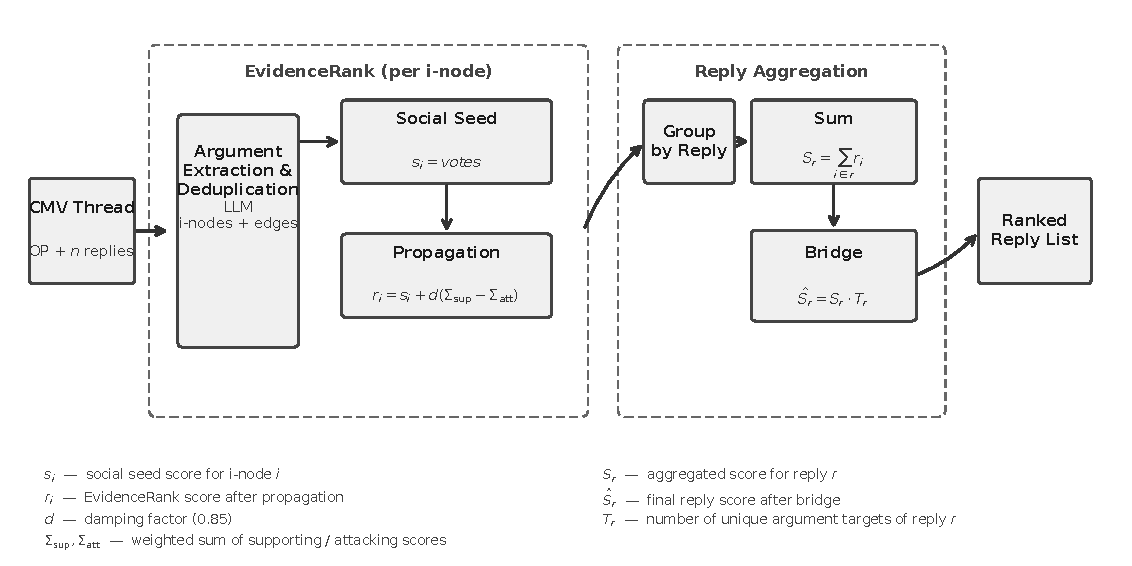
\includegraphics[width=\textwidth]{figures/architecture-er-vote-sum-nodc-bridge.pdf}
\caption{Architecture of the EvidenceRank pipeline showing argument extraction, graph propagation, and reply aggregation.}
\label{fig:architecture}
\end{figure*}


% Results and Analysis section for ArgMining paper
% Include with: % Results and Analysis section for ArgMining paper
% Include with: % Results and Analysis section for ArgMining paper
% Include with: \input{results-section}

\section{Evaluation}

We evaluate each pipeline stage independently before testing end-to-end on a reply ranking task. Full details and additional tables for the extraction and deduplication evaluations appear in Appendix~\ref{app:benchmarks}.

\subsection{Extraction and Deduplication}

\paragraph{Argument extraction.} On 90 essays from the Persuasive Essays corpus \citep{stab-gurevych-2014-annotating}, few-shot extraction achieves 0.542 F1 on I-nodes (P\,=\,0.886, R\,=\,0.403) and 0.146 F1 on S-nodes. These scores remain below supervised baselines. The LLM is conservative: when it identifies an argument, it is usually correct and well-bounded (matched-span IoU\,=\,0.932), but it misses the majority of components---particularly premises (R\,=\,0.265). Despite this, the high precision means the arguments it does extract are reliable inputs to downstream deduplication and ranking.

\paragraph{Deduplication.} On MultiPIT Expert \citep{dou-etal-2022-improving}, our retrieve-then-verify pipeline achieves F1\,=\,0.742 (P\,=\,0.663, R\,=\,0.842). Rather than the pairwise classification task proposed in the original benchmark, we evaluate a one-to-many setting where each new text is compared against all previous texts via vector retrieval followed by LLM verification---matching our deployed pipeline's operation and offering $O(n \log n)$ complexity versus $O(n^2)$ for pairwise comparison (see Appendix~\ref{app:architecture} for complexity analysis).

\subsection{End-to-End: Reply Ranking on ChangeMyView}

We evaluate on 206 threads from the Webis-CMV-20 corpus \citep{Kolyada2020}\footnote{The 206-thread count reflects the number of threads fully processed through the LLM pipeline at the time of submission; the corpus contains 3{,}051 threads with delta awards.}, where delta ($\Delta$) awards serve as explicit persuasion labels \citep{tan-etal-2016-winning}. For each thread, we exclude replies posted after the last delta award, so that only replies that could have influenced the OP are ranked. We further retain only the top 200 remaining replies by vote score; all delta-awarded replies are retained regardless of rank. This yields 6{,}096 replies of which 360 (5.9\%) received a delta award indicating successful persuasion. For each thread, we rank all replies and measure where the first delta reply appears using Mean Reciprocal Rank (MRR). Statistical significance is assessed via paired Wilcoxon signed-rank tests and paired bootstrap resampling ($n=10{,}000$), reporting the more conservative $p$-value.

\begin{table}[t]
\centering
\small
\begin{tabular}{lccc}
\toprule
\textbf{Algorithm} & \textbf{MRR} & \textbf{Hit@1} & \textbf{Sig.} \\
\midrule
Top (vote sort)          & 0.520 & 33.5\% & ---  \\
Top (reply count)        & 0.445 & ---    & **   \\
RRF(Vote+ReplyCount)     & 0.548 & ---    & ns   \\
\textbf{EvidenceRank}    & \textbf{0.590} & \textbf{42.7\%} & **   \\
\bottomrule
\end{tabular}
\caption{Reply ranking performance (206 threads). Significance vs.\ vote sort baseline: ** $p<0.01$.}
\label{tab:results}
\end{table}

EvidenceRank achieves MRR\,=\,0.590 ($p < 0.01$), placing a delta reply at rank~1 in 42.7\% of threads versus 33.5\% for vote sorting---a 27\% relative improvement (Table~\ref{tab:results}).

\subsection{Why Argument Structure Helps}

The ranking improvement is driven primarily by a simple structural signal: persuasive replies contain more arguments, consistent with prior work showing argumentation features outperform surface text features on CMV \citep{wei-etal-2016-post}. Among the 6{,}096 replies, delta replies average $5.04 \pm 2.02$ I-nodes versus $3.37 \pm 1.83$ for non-delta replies (Cohen's $d = 0.905$). I-node count alone achieves ROC~AUC\,=\,0.736 for discriminating persuasive replies, and in a logistic regression with both I-node count and child reply count as standardised predictors, I-node count has 2.5$\times$ the coefficient. EvidenceRank captures this signal through sum aggregation: replies with more extracted claims score higher, regardless of engagement. However, the large pooled effect size does not translate directly into ranking gains: within any given thread, the overlap between delta and non-delta I-node counts is substantial, limiting the per-thread discriminative power (MRR improvement +0.070, Cohen's $d = 0.187$).

This finding has a practical implication for the platform's resilience: a ranking that rewards substantive, multi-claim argumentation cannot be inflated by producing many low-quality posts. Because argument extraction is automated rather than user-labelled, gaming the ranking requires producing text that an independent LLM decomposes into multiple distinct arguments connecting to existing claims---effectively requiring the adversary to argue well. The bridge multiplier further rewards replies that engage multiple distinct points in the debate (ablation: $\Delta$MRR\,=\,+0.015 over propagation alone; see Table~\ref{tab:ablation} in Appendix~\ref{app:ablation}).

Engagement metrics, by contrast, are unreliable: sorting by child reply count performs significantly \emph{worse} than vote sorting (MRR\,=\,0.445 vs.\ 0.520, $p<0.01$), because heavily-discussed replies are often controversial rather than persuasive---consistent with \citet{tan-etal-2016-winning}'s finding that excessive back-and-forth engagement reduces persuasion success. Even combining reply count with votes via reciprocal rank fusion \citep{cormack2009reciprocal} yields no significant improvement ($p>0.05$).


\section{Evaluation}

We evaluate each pipeline stage independently before testing end-to-end on a reply ranking task. Full details and additional tables for the extraction and deduplication evaluations appear in Appendix~\ref{app:benchmarks}.

\subsection{Extraction and Deduplication}

\paragraph{Argument extraction.} On 90 essays from the Persuasive Essays corpus \citep{stab-gurevych-2014-annotating}, few-shot extraction achieves 0.542 F1 on I-nodes (P\,=\,0.886, R\,=\,0.403) and 0.146 F1 on S-nodes. These scores remain below supervised baselines. The LLM is conservative: when it identifies an argument, it is usually correct and well-bounded (matched-span IoU\,=\,0.932), but it misses the majority of components---particularly premises (R\,=\,0.265). Despite this, the high precision means the arguments it does extract are reliable inputs to downstream deduplication and ranking.

\paragraph{Deduplication.} On MultiPIT Expert \citep{dou-etal-2022-improving}, our retrieve-then-verify pipeline achieves F1\,=\,0.742 (P\,=\,0.663, R\,=\,0.842). Rather than the pairwise classification task proposed in the original benchmark, we evaluate a one-to-many setting where each new text is compared against all previous texts via vector retrieval followed by LLM verification---matching our deployed pipeline's operation and offering $O(n \log n)$ complexity versus $O(n^2)$ for pairwise comparison (see Appendix~\ref{app:architecture} for complexity analysis).

\subsection{End-to-End: Reply Ranking on ChangeMyView}

We evaluate on 206 threads from the Webis-CMV-20 corpus \citep{Kolyada2020}\footnote{The 206-thread count reflects the number of threads fully processed through the LLM pipeline at the time of submission; the corpus contains 3{,}051 threads with delta awards.}, where delta ($\Delta$) awards serve as explicit persuasion labels \citep{tan-etal-2016-winning}. For each thread, we exclude replies posted after the last delta award, so that only replies that could have influenced the OP are ranked. We further retain only the top 200 remaining replies by vote score; all delta-awarded replies are retained regardless of rank. This yields 6{,}096 replies of which 360 (5.9\%) received a delta award indicating successful persuasion. For each thread, we rank all replies and measure where the first delta reply appears using Mean Reciprocal Rank (MRR). Statistical significance is assessed via paired Wilcoxon signed-rank tests and paired bootstrap resampling ($n=10{,}000$), reporting the more conservative $p$-value.

\begin{table}[t]
\centering
\small
\begin{tabular}{lccc}
\toprule
\textbf{Algorithm} & \textbf{MRR} & \textbf{Hit@1} & \textbf{Sig.} \\
\midrule
Top (vote sort)          & 0.520 & 33.5\% & ---  \\
Top (reply count)        & 0.445 & ---    & **   \\
RRF(Vote+ReplyCount)     & 0.548 & ---    & ns   \\
\textbf{EvidenceRank}    & \textbf{0.590} & \textbf{42.7\%} & **   \\
\bottomrule
\end{tabular}
\caption{Reply ranking performance (206 threads). Significance vs.\ vote sort baseline: ** $p<0.01$.}
\label{tab:results}
\end{table}

EvidenceRank achieves MRR\,=\,0.590 ($p < 0.01$), placing a delta reply at rank~1 in 42.7\% of threads versus 33.5\% for vote sorting---a 27\% relative improvement (Table~\ref{tab:results}).

\subsection{Why Argument Structure Helps}

The ranking improvement is driven primarily by a simple structural signal: persuasive replies contain more arguments, consistent with prior work showing argumentation features outperform surface text features on CMV \citep{wei-etal-2016-post}. Among the 6{,}096 replies, delta replies average $5.04 \pm 2.02$ I-nodes versus $3.37 \pm 1.83$ for non-delta replies (Cohen's $d = 0.905$). I-node count alone achieves ROC~AUC\,=\,0.736 for discriminating persuasive replies, and in a logistic regression with both I-node count and child reply count as standardised predictors, I-node count has 2.5$\times$ the coefficient. EvidenceRank captures this signal through sum aggregation: replies with more extracted claims score higher, regardless of engagement. However, the large pooled effect size does not translate directly into ranking gains: within any given thread, the overlap between delta and non-delta I-node counts is substantial, limiting the per-thread discriminative power (MRR improvement +0.070, Cohen's $d = 0.187$).

This finding has a practical implication for the platform's resilience: a ranking that rewards substantive, multi-claim argumentation cannot be inflated by producing many low-quality posts. Because argument extraction is automated rather than user-labelled, gaming the ranking requires producing text that an independent LLM decomposes into multiple distinct arguments connecting to existing claims---effectively requiring the adversary to argue well. The bridge multiplier further rewards replies that engage multiple distinct points in the debate (ablation: $\Delta$MRR\,=\,+0.015 over propagation alone; see Table~\ref{tab:ablation} in Appendix~\ref{app:ablation}).

Engagement metrics, by contrast, are unreliable: sorting by child reply count performs significantly \emph{worse} than vote sorting (MRR\,=\,0.445 vs.\ 0.520, $p<0.01$), because heavily-discussed replies are often controversial rather than persuasive---consistent with \citet{tan-etal-2016-winning}'s finding that excessive back-and-forth engagement reduces persuasion success. Even combining reply count with votes via reciprocal rank fusion \citep{cormack2009reciprocal} yields no significant improvement ($p>0.05$).


\section{Evaluation}

We evaluate each pipeline stage independently before testing end-to-end on a reply ranking task. Full details and additional tables for the extraction and deduplication evaluations appear in Appendix~\ref{app:benchmarks}.

\subsection{Extraction and Deduplication}

\paragraph{Argument extraction.} On 90 essays from the Persuasive Essays corpus \citep{stab-gurevych-2014-annotating}, few-shot extraction achieves 0.542 F1 on I-nodes (P\,=\,0.886, R\,=\,0.403) and 0.146 F1 on S-nodes. These scores remain below supervised baselines. The LLM is conservative: when it identifies an argument, it is usually correct and well-bounded (matched-span IoU\,=\,0.932), but it misses the majority of components---particularly premises (R\,=\,0.265). Despite this, the high precision means the arguments it does extract are reliable inputs to downstream deduplication and ranking.

\paragraph{Deduplication.} On MultiPIT Expert \citep{dou-etal-2022-improving}, our retrieve-then-verify pipeline achieves F1\,=\,0.742 (P\,=\,0.663, R\,=\,0.842). Rather than the pairwise classification task proposed in the original benchmark, we evaluate a one-to-many setting where each new text is compared against all previous texts via vector retrieval followed by LLM verification---matching our deployed pipeline's operation and offering $O(n \log n)$ complexity versus $O(n^2)$ for pairwise comparison (see Appendix~\ref{app:architecture} for complexity analysis).

\subsection{End-to-End: Reply Ranking on ChangeMyView}

We evaluate on 206 threads from the Webis-CMV-20 corpus \citep{Kolyada2020}\footnote{The 206-thread count reflects the number of threads fully processed through the LLM pipeline at the time of submission; the corpus contains 3{,}051 threads with delta awards.}, where delta ($\Delta$) awards serve as explicit persuasion labels \citep{tan-etal-2016-winning}. For each thread, we exclude replies posted after the last delta award, so that only replies that could have influenced the OP are ranked. We further retain only the top 200 remaining replies by vote score; all delta-awarded replies are retained regardless of rank. This yields 6{,}096 replies of which 360 (5.9\%) received a delta award indicating successful persuasion. For each thread, we rank all replies and measure where the first delta reply appears using Mean Reciprocal Rank (MRR). Statistical significance is assessed via paired Wilcoxon signed-rank tests and paired bootstrap resampling ($n=10{,}000$), reporting the more conservative $p$-value.

\begin{table}[t]
\centering
\small
\begin{tabular}{lccc}
\toprule
\textbf{Algorithm} & \textbf{MRR} & \textbf{Hit@1} & \textbf{Sig.} \\
\midrule
Top (vote sort)          & 0.520 & 33.5\% & ---  \\
Top (reply count)        & 0.445 & ---    & **   \\
RRF(Vote+ReplyCount)     & 0.548 & ---    & ns   \\
\textbf{EvidenceRank}    & \textbf{0.590} & \textbf{42.7\%} & **   \\
\bottomrule
\end{tabular}
\caption{Reply ranking performance (206 threads). Significance vs.\ vote sort baseline: ** $p<0.01$.}
\label{tab:results}
\end{table}

EvidenceRank achieves MRR\,=\,0.590 ($p < 0.01$), placing a delta reply at rank~1 in 42.7\% of threads versus 33.5\% for vote sorting---a 27\% relative improvement (Table~\ref{tab:results}).

\subsection{Why Argument Structure Helps}

The ranking improvement is driven primarily by a simple structural signal: persuasive replies contain more arguments, consistent with prior work showing argumentation features outperform surface text features on CMV \citep{wei-etal-2016-post}. Among the 6{,}096 replies, delta replies average $5.04 \pm 2.02$ I-nodes versus $3.37 \pm 1.83$ for non-delta replies (Cohen's $d = 0.905$). I-node count alone achieves ROC~AUC\,=\,0.736 for discriminating persuasive replies, and in a logistic regression with both I-node count and child reply count as standardised predictors, I-node count has 2.5$\times$ the coefficient. EvidenceRank captures this signal through sum aggregation: replies with more extracted claims score higher, regardless of engagement. However, the large pooled effect size does not translate directly into ranking gains: within any given thread, the overlap between delta and non-delta I-node counts is substantial, limiting the per-thread discriminative power (MRR improvement +0.070, Cohen's $d = 0.187$).

This finding has a practical implication for the platform's resilience: a ranking that rewards substantive, multi-claim argumentation cannot be inflated by producing many low-quality posts. Because argument extraction is automated rather than user-labelled, gaming the ranking requires producing text that an independent LLM decomposes into multiple distinct arguments connecting to existing claims---effectively requiring the adversary to argue well. The bridge multiplier further rewards replies that engage multiple distinct points in the debate (ablation: $\Delta$MRR\,=\,+0.015 over propagation alone; see Table~\ref{tab:ablation} in Appendix~\ref{app:ablation}).

Engagement metrics, by contrast, are unreliable: sorting by child reply count performs significantly \emph{worse} than vote sorting (MRR\,=\,0.445 vs.\ 0.520, $p<0.01$), because heavily-discussed replies are often controversial rather than persuasive---consistent with \citet{tan-etal-2016-winning}'s finding that excessive back-and-forth engagement reduces persuasion success. Even combining reply count with votes via reciprocal rank fusion \citep{cormack2009reciprocal} yields no significant improvement ($p>0.05$).


% Conclusion section for ArgMining paper
% Include with: % Conclusion section for ArgMining paper
% Include with: % Conclusion section for ArgMining paper
% Include with: \input{conclusion-section}

\section{Conclusion}

We presented an end-to-end LLM-powered pipeline that transforms social media discussions into structured argument graphs using only few-shot prompting. Despite extraction recall limitations (particularly on premises) and weak relation detection, the pipeline produces structure that is precise enough to significantly improve reply ranking over vote sorting on ChangeMyView (MRR 0.590 vs.\ 0.520, $p<0.01$).

The key finding is that LLM-extracted argument counts---a signal unavailable without automated mining---are more predictive of persuasion than engagement metrics. By combining this structural signal with social votes, EvidenceRank rewards substantive, multi-claim argumentation in a way that is difficult to game without arguing well. This property is essential for platforms that aim to integrate machine participants alongside humans.

Future work should address the pipeline's main bottleneck---low premise recall---through domain-specific fine-tuning or hybrid architectures, and test whether these findings generalise beyond the explicit argumentation norms of ChangeMyView to less structured deliberative settings.


\section{Conclusion}

We presented an end-to-end LLM-powered pipeline that transforms social media discussions into structured argument graphs using only few-shot prompting. Despite extraction recall limitations (particularly on premises) and weak relation detection, the pipeline produces structure that is precise enough to significantly improve reply ranking over vote sorting on ChangeMyView (MRR 0.590 vs.\ 0.520, $p<0.01$).

The key finding is that LLM-extracted argument counts---a signal unavailable without automated mining---are more predictive of persuasion than engagement metrics. By combining this structural signal with social votes, EvidenceRank rewards substantive, multi-claim argumentation in a way that is difficult to game without arguing well. This property is essential for platforms that aim to integrate machine participants alongside humans.

Future work should address the pipeline's main bottleneck---low premise recall---through domain-specific fine-tuning or hybrid architectures, and test whether these findings generalise beyond the explicit argumentation norms of ChangeMyView to less structured deliberative settings.


\section{Conclusion}

We presented an end-to-end LLM-powered pipeline that transforms social media discussions into structured argument graphs using only few-shot prompting. Despite extraction recall limitations (particularly on premises) and weak relation detection, the pipeline produces structure that is precise enough to significantly improve reply ranking over vote sorting on ChangeMyView (MRR 0.590 vs.\ 0.520, $p<0.01$).

The key finding is that LLM-extracted argument counts---a signal unavailable without automated mining---are more predictive of persuasion than engagement metrics. By combining this structural signal with social votes, EvidenceRank rewards substantive, multi-claim argumentation in a way that is difficult to game without arguing well. This property is essential for platforms that aim to integrate machine participants alongside humans.

Future work should address the pipeline's main bottleneck---low premise recall---through domain-specific fine-tuning or hybrid architectures, and test whether these findings generalise beyond the explicit argumentation norms of ChangeMyView to less structured deliberative settings.


% Limitations section for ArgMining paper
% Include with: % Limitations section for ArgMining paper
% Include with: % Limitations section for ArgMining paper
% Include with: \input{limitations-section}
% Does not count towards page limit.

\section*{Limitations}

Our extraction pipeline has low recall, particularly on premises (R\,=\,0.265), meaning the LLM misses the majority of argumentative units---bounded by what few-shot prompting can achieve without fine-tuning. S-node detection is weak end-to-end (F1\,=\,0.146), though this metric conflates missed I-nodes (which make their incident edges unmatchable) with missed relations between correctly detected I-nodes; the conditional accuracy of relation detection given correctly extracted endpoints is not measured. Extraction was evaluated only on formal text (Persuasive Essays), so performance on informal social media text is unknown. Deduplication precision of 0.663 means roughly one in three merges is incorrect, potentially conflating distinct arguments, and was evaluated on Twitter paraphrases (MultiPIT) rather than argumentative text specifically.

The end-to-end evaluation has several constraints. The effect size is small (Cohen's $d$\,=\,0.187), and EvidenceRank produces the same ranking as vote sorting in approximately 40\% of threads. We evaluate on a single corpus of 206 CMV threads, which has explicit argumentation norms and a built-in persuasion signal that may not generalise to other settings. Delta awards are noisy and discretionary; threads may contain persuasive replies that never received a delta. Each thread is processed independently, yielding small, isolated argument graphs; a deployed platform with accumulated cross-thread deduplication would have much denser graphs, and EvidenceRank's propagation could behave differently at that density.

Finally, the pipeline requires multiple LLM API calls per post (extraction plus deduplication candidates), which is expensive at scale and may not suit real-time ranking. Our claim that argument-quality ranking is resilient to manipulation is architectural and has not been verified through adversarial experiments.

% Does not count towards page limit.

\section*{Limitations}

Our extraction pipeline has low recall, particularly on premises (R\,=\,0.265), meaning the LLM misses the majority of argumentative units---bounded by what few-shot prompting can achieve without fine-tuning. S-node detection is weak end-to-end (F1\,=\,0.146), though this metric conflates missed I-nodes (which make their incident edges unmatchable) with missed relations between correctly detected I-nodes; the conditional accuracy of relation detection given correctly extracted endpoints is not measured. Extraction was evaluated only on formal text (Persuasive Essays), so performance on informal social media text is unknown. Deduplication precision of 0.663 means roughly one in three merges is incorrect, potentially conflating distinct arguments, and was evaluated on Twitter paraphrases (MultiPIT) rather than argumentative text specifically.

The end-to-end evaluation has several constraints. The effect size is small (Cohen's $d$\,=\,0.187), and EvidenceRank produces the same ranking as vote sorting in approximately 40\% of threads. We evaluate on a single corpus of 206 CMV threads, which has explicit argumentation norms and a built-in persuasion signal that may not generalise to other settings. Delta awards are noisy and discretionary; threads may contain persuasive replies that never received a delta. Each thread is processed independently, yielding small, isolated argument graphs; a deployed platform with accumulated cross-thread deduplication would have much denser graphs, and EvidenceRank's propagation could behave differently at that density.

Finally, the pipeline requires multiple LLM API calls per post (extraction plus deduplication candidates), which is expensive at scale and may not suit real-time ranking. Our claim that argument-quality ranking is resilient to manipulation is architectural and has not been verified through adversarial experiments.

% Does not count towards page limit.

\section*{Limitations}

Our extraction pipeline has low recall, particularly on premises (R\,=\,0.265), meaning the LLM misses the majority of argumentative units---bounded by what few-shot prompting can achieve without fine-tuning. S-node detection is weak end-to-end (F1\,=\,0.146), though this metric conflates missed I-nodes (which make their incident edges unmatchable) with missed relations between correctly detected I-nodes; the conditional accuracy of relation detection given correctly extracted endpoints is not measured. Extraction was evaluated only on formal text (Persuasive Essays), so performance on informal social media text is unknown. Deduplication precision of 0.663 means roughly one in three merges is incorrect, potentially conflating distinct arguments, and was evaluated on Twitter paraphrases (MultiPIT) rather than argumentative text specifically.

The end-to-end evaluation has several constraints. The effect size is small (Cohen's $d$\,=\,0.187), and EvidenceRank produces the same ranking as vote sorting in approximately 40\% of threads. We evaluate on a single corpus of 206 CMV threads, which has explicit argumentation norms and a built-in persuasion signal that may not generalise to other settings. Delta awards are noisy and discretionary; threads may contain persuasive replies that never received a delta. Each thread is processed independently, yielding small, isolated argument graphs; a deployed platform with accumulated cross-thread deduplication would have much denser graphs, and EvidenceRank's propagation could behave differently at that density.

Finally, the pipeline requires multiple LLM API calls per post (extraction plus deduplication candidates), which is expensive at scale and may not suit real-time ranking. Our claim that argument-quality ranking is resilient to manipulation is architectural and has not been verified through adversarial experiments.


\section*{Ethical Considerations}
% Ethical Considerations section for ArgMining paper
% Include with: % Ethical Considerations section for ArgMining paper
% Include with: % Ethical Considerations section for ArgMining paper
% Include with: \input{ethical-considerations-section} after \section*{Ethical Considerations}

\begin{itemize}[leftmargin=*,nosep]

\item \textbf{Ranking as curation.} Deciding which arguments people see and interact with is a fundamentally different ethical problem than identifying what arguments people have made. Defining argument quality algorithmically is inherently normative: by privileging some types of arguments (multi-claim structured argumentation), we disadvantage other arguments (simple and concrete arguments). Well-structured propaganda could rank highly regardless of truthfulness \citep{verma-etal-2025-reasoning-rhetoric}, because no algorithm is completely immune to intentionally bad inputs.

\item \textbf{LLM bias.} The pipeline inherits the biases of its underlying LLMs \citep{bender-etal-2021-stochastic-parrots}. Extraction and deduplication may systematically favor certain rhetorical styles over other equally valid arguments. Deduplication merges risk collapsing minority viewpoints into majority framings. Any systematic bias will have a disparate impact across user populations.

\item \textbf{Human-AI interaction.} Enabling AI agents to participate alongside humans raises disclosure questions---users should know which contributions are machine-generated. AI agents can produce high-volume, multi-claim arguments effortlessly, creating an asymmetry that risks displacing human deliberation. Our tools are designed to assist and augment human reasoning, not to replace it.

\item \textbf{Data and privacy.} Our ChangeMyView evaluation uses publicly available Reddit data whose authors did not specifically consent to argument mining research \citep{gliniecka-2023-situated-ethics-reddit}. In production, users could import data from other media where users/authors who may not have specifically consented. More broadly, structured argument graphs make users' reasoning patterns more visible and trackable than raw text, and cross-thread deduplication creates a map of who argues what across discussions.

\item \textbf{Dual-use risks.} The same argument mining technology that can foster healthier discourse could be misused---for example, to identify and suppress dissenting arguments, or to optimize propaganda for high ranking. More broadly, algorithmic mediation of discourse risks depoliticisation even when well-intentioned \citep{oleart-palomo-2025-technosolutionism}, and our resilience claims regarding manipulation are preliminary.

\item \textbf{Cost and access.} Dependency on commercial LLM APIs means the platform's core analytical function is controlled by a third party. The cost of LLM calls per post creates a barrier---argument-quality ranking may only be feasible for well-funded platforms, raising questions about equitable access to these tools.

\item \textbf{Positive potential.} Ranking by argument substance rather than engagement metrics offers an alternative to advertising-driven platforms that optimize for time-on-platform. Making argument structure visible and navigable supports deliberative democracy, and transparent, open ranking algorithms allow public scrutiny of how content is surfaced. Structured argument graphs can also serve as autodidactic resources, providing users with feedback on the structure and epistemic status of their reasoning. More broadly, QBAFs have shown promise for truth discovery in multi-source settings \citep{potyka-booth-2022-td-qbaf}; with improved architectures, platforms built on argument graphs could move beyond relevance and persuasiveness toward surfacing reliable knowledge.

\end{itemize}
 after \section*{Ethical Considerations}

\begin{itemize}[leftmargin=*,nosep]

\item \textbf{Ranking as curation.} Deciding which arguments people see and interact with is a fundamentally different ethical problem than identifying what arguments people have made. Defining argument quality algorithmically is inherently normative: by privileging some types of arguments (multi-claim structured argumentation), we disadvantage other arguments (simple and concrete arguments). Well-structured propaganda could rank highly regardless of truthfulness \citep{verma-etal-2025-reasoning-rhetoric}, because no algorithm is completely immune to intentionally bad inputs.

\item \textbf{LLM bias.} The pipeline inherits the biases of its underlying LLMs \citep{bender-etal-2021-stochastic-parrots}. Extraction and deduplication may systematically favor certain rhetorical styles over other equally valid arguments. Deduplication merges risk collapsing minority viewpoints into majority framings. Any systematic bias will have a disparate impact across user populations.

\item \textbf{Human-AI interaction.} Enabling AI agents to participate alongside humans raises disclosure questions---users should know which contributions are machine-generated. AI agents can produce high-volume, multi-claim arguments effortlessly, creating an asymmetry that risks displacing human deliberation. Our tools are designed to assist and augment human reasoning, not to replace it.

\item \textbf{Data and privacy.} Our ChangeMyView evaluation uses publicly available Reddit data whose authors did not specifically consent to argument mining research \citep{gliniecka-2023-situated-ethics-reddit}. In production, users could import data from other media where users/authors who may not have specifically consented. More broadly, structured argument graphs make users' reasoning patterns more visible and trackable than raw text, and cross-thread deduplication creates a map of who argues what across discussions.

\item \textbf{Dual-use risks.} The same argument mining technology that can foster healthier discourse could be misused---for example, to identify and suppress dissenting arguments, or to optimize propaganda for high ranking. More broadly, algorithmic mediation of discourse risks depoliticisation even when well-intentioned \citep{oleart-palomo-2025-technosolutionism}, and our resilience claims regarding manipulation are preliminary.

\item \textbf{Cost and access.} Dependency on commercial LLM APIs means the platform's core analytical function is controlled by a third party. The cost of LLM calls per post creates a barrier---argument-quality ranking may only be feasible for well-funded platforms, raising questions about equitable access to these tools.

\item \textbf{Positive potential.} Ranking by argument substance rather than engagement metrics offers an alternative to advertising-driven platforms that optimize for time-on-platform. Making argument structure visible and navigable supports deliberative democracy, and transparent, open ranking algorithms allow public scrutiny of how content is surfaced. Structured argument graphs can also serve as autodidactic resources, providing users with feedback on the structure and epistemic status of their reasoning. More broadly, QBAFs have shown promise for truth discovery in multi-source settings \citep{potyka-booth-2022-td-qbaf}; with improved architectures, platforms built on argument graphs could move beyond relevance and persuasiveness toward surfacing reliable knowledge.

\end{itemize}
 after \section*{Ethical Considerations}

\begin{itemize}[leftmargin=*,nosep]

\item \textbf{Ranking as curation.} Deciding which arguments people see and interact with is a fundamentally different ethical problem than identifying what arguments people have made. Defining argument quality algorithmically is inherently normative: by privileging some types of arguments (multi-claim structured argumentation), we disadvantage other arguments (simple and concrete arguments). Well-structured propaganda could rank highly regardless of truthfulness \citep{verma-etal-2025-reasoning-rhetoric}, because no algorithm is completely immune to intentionally bad inputs.

\item \textbf{LLM bias.} The pipeline inherits the biases of its underlying LLMs \citep{bender-etal-2021-stochastic-parrots}. Extraction and deduplication may systematically favor certain rhetorical styles over other equally valid arguments. Deduplication merges risk collapsing minority viewpoints into majority framings. Any systematic bias will have a disparate impact across user populations.

\item \textbf{Human-AI interaction.} Enabling AI agents to participate alongside humans raises disclosure questions---users should know which contributions are machine-generated. AI agents can produce high-volume, multi-claim arguments effortlessly, creating an asymmetry that risks displacing human deliberation. Our tools are designed to assist and augment human reasoning, not to replace it.

\item \textbf{Data and privacy.} Our ChangeMyView evaluation uses publicly available Reddit data whose authors did not specifically consent to argument mining research \citep{gliniecka-2023-situated-ethics-reddit}. In production, users could import data from other media where users/authors who may not have specifically consented. More broadly, structured argument graphs make users' reasoning patterns more visible and trackable than raw text, and cross-thread deduplication creates a map of who argues what across discussions.

\item \textbf{Dual-use risks.} The same argument mining technology that can foster healthier discourse could be misused---for example, to identify and suppress dissenting arguments, or to optimize propaganda for high ranking. More broadly, algorithmic mediation of discourse risks depoliticisation even when well-intentioned \citep{oleart-palomo-2025-technosolutionism}, and our resilience claims regarding manipulation are preliminary.

\item \textbf{Cost and access.} Dependency on commercial LLM APIs means the platform's core analytical function is controlled by a third party. The cost of LLM calls per post creates a barrier---argument-quality ranking may only be feasible for well-funded platforms, raising questions about equitable access to these tools.

\item \textbf{Positive potential.} Ranking by argument substance rather than engagement metrics offers an alternative to advertising-driven platforms that optimize for time-on-platform. Making argument structure visible and navigable supports deliberative democracy, and transparent, open ranking algorithms allow public scrutiny of how content is surfaced. Structured argument graphs can also serve as autodidactic resources, providing users with feedback on the structure and epistemic status of their reasoning. More broadly, QBAFs have shown promise for truth discovery in multi-source settings \citep{potyka-booth-2022-td-qbaf}; with improved architectures, platforms built on argument graphs could move beyond relevance and persuasiveness toward surfacing reliable knowledge.

\end{itemize}


\section*{Acknowledgments}
% Acknowledgments section for ArgMining paper
% Include with: % Acknowledgments section for ArgMining paper
% Include with: % Acknowledgments section for ArgMining paper
% Include with: \input{acknowledgments-section} inside \section*{Acknowledgments}

Generative AI tools were used to assist with literature search,
generation of research ideas and framing, drafting of section text
from author-specified ideas and results, and language polishing.
The underlying platform code was also generated with AI assistance.
All generated content was reviewed and verified by the authors,
who take full responsibility for the paper's content.
 inside \section*{Acknowledgments}

Generative AI tools were used to assist with literature search,
generation of research ideas and framing, drafting of section text
from author-specified ideas and results, and language polishing.
The underlying platform code was also generated with AI assistance.
All generated content was reviewed and verified by the authors,
who take full responsibility for the paper's content.
 inside \section*{Acknowledgments}

Generative AI tools were used to assist with literature search,
generation of research ideas and framing, drafting of section text
from author-specified ideas and results, and language polishing.
The underlying platform code was also generated with AI assistance.
All generated content was reviewed and verified by the authors,
who take full responsibility for the paper's content.


% Bibliography entries for the entire Anthology, followed by custom entries
%\bibliography{anthology,custom}
% Custom bibliography entries only
\bibliography{custom}

\appendix
% Appendix section for ArgMining paper
% Include with: \appendix % Appendix section for ArgMining paper
% Include with: \appendix % Appendix section for ArgMining paper
% Include with: \appendix \input{appendix-section}

\section{Complexity Analysis}
\label{app:architecture}

Let $N$ denote the number of I-nodes, $E$ the number of edges, $K$ the number of propagation iterations (fixed at 20), and $R$ the number of replies. EvidenceRank propagation runs in $O(K(N + E))$, which simplifies to $O(N + E)$ for fixed $K$---analogous to PageRank on a sparse graph. Reply aggregation and bridge multiplier computation are $O(N + E)$, and the final sort is $O(R \log R)$. The full ranking pipeline is $O(N + E + R \log R)$; since typically $E > N \geq R$ in argumentation graphs, the practical complexity is $O(E)$. For deduplication, each new I-node requires one embedding, one HNSW search ($O(\log |\mathcal{N}|)$), and one LLM verification call, giving $O(|\mathcal{N}|)$ total calls for $|\mathcal{N}|$ I-nodes processed incrementally---versus $O(|\mathcal{N}|^2)$ for pairwise comparison.

\section{Benchmark Details}
\label{app:benchmarks}

Table~\ref{tab:extraction} reports extraction performance by component type on 90 essays from \citet{stab-gurevych-2014-annotating}. A span is considered matched if the IoU with a ground-truth span exceeds 0.5.

\begin{table}[ht]
\centering
\small
\begin{tabular}{lccc}
\toprule
\textbf{Component Type} & \textbf{P} & \textbf{R} & \textbf{F1} \\
\midrule
Major Claim & 1.000 & 0.733 & 0.846 \\
Claim       & 1.000 & 0.534 & 0.696 \\
Premise     & 1.000 & 0.265 & 0.419 \\
\midrule
All I-nodes & 0.886 & 0.403 & 0.542 \\
S-nodes     & 0.303 & 0.101 & 0.146 \\
\bottomrule
\end{tabular}
\caption{Extraction performance by component type on the Persuasive Essays corpus. Span IoU threshold = 0.5; matched-span IoU = 0.932; role alignment = 67.0\%.}
\label{tab:extraction}
\end{table}

Table~\ref{tab:dedup} reports deduplication performance on MultiPIT Expert \citep{dou-etal-2022-improving} (557 sentence pairs: 254 positive, 303 negative).

\begin{table}[ht]
\centering
\small
\begin{tabular}{lr}
\toprule
\textbf{Metric} & \textbf{Value} \\
\midrule
Precision & 0.663 \\
Recall    & 0.842 \\
F1        & 0.742 \\
Accuracy  & 0.732 \\
\midrule
TP / FP / FN / TN & 214 / 109 / 40 / 194 \\
\bottomrule
\end{tabular}
\caption{Deduplication performance on MultiPIT Expert.}
\label{tab:dedup}
\end{table}

\section{Ablation Study}
\label{app:ablation}

Table~\ref{tab:ablation} traces the contribution of each pipeline component. Sum aggregation with graph propagation provides the primary improvement over vote sorting ($\Delta$MRR +0.055, $p < 0.001$). The bridge multiplier contributes a further +0.015, though this increment is not individually significant ($p = 0.56$ vs.\ the no-bridge variant).

\begin{table}[ht]
\centering
\footnotesize
\begin{tabular}{lccc}
\toprule
\textbf{Configuration} & \textbf{MRR} & \textbf{$\Delta$MRR} & \textbf{Sig.} \\
\midrule
Vote sort              & 0.520 & ---            & ---  \\
+ Prop.\ + Sum agg.   & 0.575 & +0.055         & $p{<}0.001$   \\
+ Bridge mult.         & \textbf{0.590} & \textbf{+0.070} & $p{<}0.01$   \\
\bottomrule
\end{tabular}
\caption{Ablation study. Each row adds one component to the pipeline. $\Delta$MRR is measured against the vote sort baseline. Significance is assessed via paired Wilcoxon signed-rank test vs.\ the vote sort baseline.}
\label{tab:ablation}
\end{table}


\section{Complexity Analysis}
\label{app:architecture}

Let $N$ denote the number of I-nodes, $E$ the number of edges, $K$ the number of propagation iterations (fixed at 20), and $R$ the number of replies. EvidenceRank propagation runs in $O(K(N + E))$, which simplifies to $O(N + E)$ for fixed $K$---analogous to PageRank on a sparse graph. Reply aggregation and bridge multiplier computation are $O(N + E)$, and the final sort is $O(R \log R)$. The full ranking pipeline is $O(N + E + R \log R)$; since typically $E > N \geq R$ in argumentation graphs, the practical complexity is $O(E)$. For deduplication, each new I-node requires one embedding, one HNSW search ($O(\log |\mathcal{N}|)$), and one LLM verification call, giving $O(|\mathcal{N}|)$ total calls for $|\mathcal{N}|$ I-nodes processed incrementally---versus $O(|\mathcal{N}|^2)$ for pairwise comparison.

\section{Benchmark Details}
\label{app:benchmarks}

Table~\ref{tab:extraction} reports extraction performance by component type on 90 essays from \citet{stab-gurevych-2014-annotating}. A span is considered matched if the IoU with a ground-truth span exceeds 0.5.

\begin{table}[ht]
\centering
\small
\begin{tabular}{lccc}
\toprule
\textbf{Component Type} & \textbf{P} & \textbf{R} & \textbf{F1} \\
\midrule
Major Claim & 1.000 & 0.733 & 0.846 \\
Claim       & 1.000 & 0.534 & 0.696 \\
Premise     & 1.000 & 0.265 & 0.419 \\
\midrule
All I-nodes & 0.886 & 0.403 & 0.542 \\
S-nodes     & 0.303 & 0.101 & 0.146 \\
\bottomrule
\end{tabular}
\caption{Extraction performance by component type on the Persuasive Essays corpus. Span IoU threshold = 0.5; matched-span IoU = 0.932; role alignment = 67.0\%.}
\label{tab:extraction}
\end{table}

Table~\ref{tab:dedup} reports deduplication performance on MultiPIT Expert \citep{dou-etal-2022-improving} (557 sentence pairs: 254 positive, 303 negative).

\begin{table}[ht]
\centering
\small
\begin{tabular}{lr}
\toprule
\textbf{Metric} & \textbf{Value} \\
\midrule
Precision & 0.663 \\
Recall    & 0.842 \\
F1        & 0.742 \\
Accuracy  & 0.732 \\
\midrule
TP / FP / FN / TN & 214 / 109 / 40 / 194 \\
\bottomrule
\end{tabular}
\caption{Deduplication performance on MultiPIT Expert.}
\label{tab:dedup}
\end{table}

\section{Ablation Study}
\label{app:ablation}

Table~\ref{tab:ablation} traces the contribution of each pipeline component. Sum aggregation with graph propagation provides the primary improvement over vote sorting ($\Delta$MRR +0.055, $p < 0.001$). The bridge multiplier contributes a further +0.015, though this increment is not individually significant ($p = 0.56$ vs.\ the no-bridge variant).

\begin{table}[ht]
\centering
\footnotesize
\begin{tabular}{lccc}
\toprule
\textbf{Configuration} & \textbf{MRR} & \textbf{$\Delta$MRR} & \textbf{Sig.} \\
\midrule
Vote sort              & 0.520 & ---            & ---  \\
+ Prop.\ + Sum agg.   & 0.575 & +0.055         & $p{<}0.001$   \\
+ Bridge mult.         & \textbf{0.590} & \textbf{+0.070} & $p{<}0.01$   \\
\bottomrule
\end{tabular}
\caption{Ablation study. Each row adds one component to the pipeline. $\Delta$MRR is measured against the vote sort baseline. Significance is assessed via paired Wilcoxon signed-rank test vs.\ the vote sort baseline.}
\label{tab:ablation}
\end{table}


\section{Complexity Analysis}
\label{app:architecture}

Let $N$ denote the number of I-nodes, $E$ the number of edges, $K$ the number of propagation iterations (fixed at 20), and $R$ the number of replies. EvidenceRank propagation runs in $O(K(N + E))$, which simplifies to $O(N + E)$ for fixed $K$---analogous to PageRank on a sparse graph. Reply aggregation and bridge multiplier computation are $O(N + E)$, and the final sort is $O(R \log R)$. The full ranking pipeline is $O(N + E + R \log R)$; since typically $E > N \geq R$ in argumentation graphs, the practical complexity is $O(E)$. For deduplication, each new I-node requires one embedding, one HNSW search ($O(\log |\mathcal{N}|)$), and one LLM verification call, giving $O(|\mathcal{N}|)$ total calls for $|\mathcal{N}|$ I-nodes processed incrementally---versus $O(|\mathcal{N}|^2)$ for pairwise comparison.

\section{Benchmark Details}
\label{app:benchmarks}

Table~\ref{tab:extraction} reports extraction performance by component type on 90 essays from \citet{stab-gurevych-2014-annotating}. A span is considered matched if the IoU with a ground-truth span exceeds 0.5.

\begin{table}[ht]
\centering
\small
\begin{tabular}{lccc}
\toprule
\textbf{Component Type} & \textbf{P} & \textbf{R} & \textbf{F1} \\
\midrule
Major Claim & 1.000 & 0.733 & 0.846 \\
Claim       & 1.000 & 0.534 & 0.696 \\
Premise     & 1.000 & 0.265 & 0.419 \\
\midrule
All I-nodes & 0.886 & 0.403 & 0.542 \\
S-nodes     & 0.303 & 0.101 & 0.146 \\
\bottomrule
\end{tabular}
\caption{Extraction performance by component type on the Persuasive Essays corpus. Span IoU threshold = 0.5; matched-span IoU = 0.932; role alignment = 67.0\%.}
\label{tab:extraction}
\end{table}

Table~\ref{tab:dedup} reports deduplication performance on MultiPIT Expert \citep{dou-etal-2022-improving} (557 sentence pairs: 254 positive, 303 negative).

\begin{table}[ht]
\centering
\small
\begin{tabular}{lr}
\toprule
\textbf{Metric} & \textbf{Value} \\
\midrule
Precision & 0.663 \\
Recall    & 0.842 \\
F1        & 0.742 \\
Accuracy  & 0.732 \\
\midrule
TP / FP / FN / TN & 214 / 109 / 40 / 194 \\
\bottomrule
\end{tabular}
\caption{Deduplication performance on MultiPIT Expert.}
\label{tab:dedup}
\end{table}

\section{Ablation Study}
\label{app:ablation}

Table~\ref{tab:ablation} traces the contribution of each pipeline component. Sum aggregation with graph propagation provides the primary improvement over vote sorting ($\Delta$MRR +0.055, $p < 0.001$). The bridge multiplier contributes a further +0.015, though this increment is not individually significant ($p = 0.56$ vs.\ the no-bridge variant).

\begin{table}[ht]
\centering
\footnotesize
\begin{tabular}{lccc}
\toprule
\textbf{Configuration} & \textbf{MRR} & \textbf{$\Delta$MRR} & \textbf{Sig.} \\
\midrule
Vote sort              & 0.520 & ---            & ---  \\
+ Prop.\ + Sum agg.   & 0.575 & +0.055         & $p{<}0.001$   \\
+ Bridge mult.         & \textbf{0.590} & \textbf{+0.070} & $p{<}0.01$   \\
\bottomrule
\end{tabular}
\caption{Ablation study. Each row adds one component to the pipeline. $\Delta$MRR is measured against the vote sort baseline. Significance is assessed via paired Wilcoxon signed-rank test vs.\ the vote sort baseline.}
\label{tab:ablation}
\end{table}


\end{document}
